\documentclass[fontsize=12pt,BCOR=5mm,DIV=12,
               parskip=half,
               listof=entryprefix,paper=a4,toc=bibliography,toc=listof,pointlessnumbers
               ]{scrreprt}

%%%%%%%%%%%%%%%%%%%%%%%%%%%%%%% PACKAGES %%%%%%%%%%%%%%%%%%%%%%%%%%%%%%

\usepackage{graphicx}
\usepackage{csvsimple}
\usepackage{tabularx}
\usepackage{booktabs}
\usepackage{minted}
\usepackage{amsmath}
\usepackage{csquotes}
\usepackage{caption}
\usepackage[linguistics]{forest} % Für das Zeichnen von Entscheidungsbäumen
\usepackage[hidelinks]{hyperref} % Macht Referenzen anklickbar
\usepackage{fancyhdr} % Kaitel und Sektionen werden im Header einer Seite angezeigt


%%%% LANGUAGE PACKAGES %%%%
\usepackage[utf8]{inputenc}
\usepackage[ngerman]{babel} % Übersetzung der Dokumentteile z.B. Figure zu Abbildung

%%%%%%%%%%%%%%%%%%%%%%%%%%%%%%% BIB SETUP %%%%%%%%%%%%%%%%%%%%%%%%%%%%%%

\usepackage[
	backend=biber,
	style=ieee,
	natbib=true,
	url=true, 
	doi=true,
	eprint=false
]{biblatex}
\addbibresource{./bibliography/bibliography.bib}

%%%%%%%%%%%%%%%%%%%%%%%%%%%%%%%% VARS AND CONFIG %%%%%%%%%%%%%%%%%%%%%%%%%%%%%%%%%%

\graphicspath{{./img}}
\setcounter{tocdepth}{1} % Regelt welche Überschriftstiefe im Inhaltverz. angezeigt wird
\pagestyle{fancy} % Kaitel und Sektionen werden im Header einer Seite angezeigt

%%%%%%%%%%%%%%%%%%%%%%%%%%%%%%%%%%%%%%%%%%%%%%%%%%%%%%%%%%%%%%%%%%%%%%%
%%%%%%%%%%%%%%%%%%%%%%%%%%%%%%%% DOC %%%%%%%%%%%%%%%%%%%%%%%%%%%%%%%%%%
%%%%%%%%%%%%%%%%%%%%%%%%%%%%%%%%%%%%%%%%%%%%%%%%%%%%%%%%%%%%%%%%%%%%%%%

\begin{document}
  
%%% CONTENT %%%

\begin{titlepage}
    \begin{minipage}{\textwidth}
        \vspace{-2cm}
        
\includegraphics{logo-dhbw.pdf}
    \end{minipage}
    \vspace{1em}

    \begin{center}
		{\textsf{\large Duale Hochschule Baden - W\"urttemberg Mannheim}}\\[4em]
		{\textsf{\textbf{\large{Seminararbeit}}}}\\[6mm]                                 % Art der Arbeit
		{\textsf{\textbf{\Large{Entscheidungsbäume}}}} \\[0.5cm]                        % Titel der Arbeit
		{\textsf{Am Beispiel des ID3 Algorithmus}} \\[1.5cm]
		{\textsf{\textbf{\large{Studiengang Angewandte Informatik}}}}\\[6mm]
		{\textsf{\textbf{Studienrichtung Informatik}}}\vspace{12em}
		\begin{minipage}{\textwidth}
			\begin{tabbing}
				Wissenschaftliche(r) Betreuer(in): \hspace{0.85cm}\=\kill
				Autor: \> Martin Pretz \\[1.5mm]
				Matrikelnummer: \> 7060026 \\[1.5mm]
				Kurs: \> TINF18AI1 \\[1.5mm]
				%Studiengangsleiter: \> \DerStudiengangsleiter \\[1.5mm]
				%Wissenschaftliche(r) Betreuer(in): \> \DerWissBetreuer \\[1.5mm]
				Bearbeitungszeitraum: \> 19.05.2021 - 10.06.2021 \\[1.5mm]
				%		alternativ:\\[1.5mm]
				%		Eingereicht: \> \DasAbgabedatum	
			\end{tabbing}
		\end{minipage}
	\end{center}
\end{titlepage}
\chapter*{Ehrenwörtliche Erklärung}
\label{ewerkl}

Ich versichere hiermit, dass ich die vorliegende Arbeit mit dem Thema: \textit{Entscheidungsbäume - Am Beispiel des ID3 Algorithmus} selbstständig verfasst und keine anderen, als die angegebenen Quellen und Hilfsmittel benutzt habe.

\vspace{1cm}
\begin{figure*}[h]
    \includegraphics[width=0.2\textwidth]{img/Unterschrift.png}
\end{figure*}

\begin{tabularx}{\textwidth}[b]{p{5cm} X p{1cm}} \cline{1-1}
    \vspace{.1cm}
    Martin Pretz
\end{tabularx}

%%% Verzeichnisse %%%
\tableofcontents % Inhaltsverzeichnis
\listoffigures % Abbildungsverzeichnis
\listoftables % Tabellenverzeichnis


\chapter{Abstract}
\label{abstract}
\chapter{Einführung}
\label{einfuehrung}

Die Frage nach der korrekten Entscheidung bzw. die Herausforderung eine korrekte Vorhersage für ein Ereignis zu treffen beschäftigt sowohl Ökonomen als auch Wissenschaftler. Zum Beispiel stellt sich die Frage ob der Kurs eines bestimmten Wertpapiers in nächster Zeit steigen oder fallen wird oder ob eine bestimmte Behandlung für einen Patienten empfehlenswert ist. \autocite{QuinlanDecisionTrees}
Zu diesem Zweck kommt unter anderem künstliche Intelligenz zum Einsatz, konkret kommt hierbei besonders maschinelles Lernen im Form der Klassifikation zum Einsatz. \autocite{QuinlanID3} Dabei wird versucht eine Vorhersage anhand von vergangenen Erfahrungen bzw. Daten vorzunehmen, es wird also eine Größe unter Berücksichtigung von verschiedenen Variablen vorhergesagt. Dafür können verschiedene Methoden zum Einsatz kommen, wobei Entscheidungsbäume eine der bekanntesten Methode ist. Daher werden in dieser Arbeit Entscheidungsbäume näher beleuchtet.
\chapter{Was sind Entscheidungsbäume?}
\label{eb:was-sind-entscheidungsbaeume}

\section{Aufbau und Funtionsweise}
\label{eb:aufbau}
Ein Entscheidungsbaum ist ein geordneter und gerichteter \autocite{DataMining} Baum welcher aus Knoten und Kanten besteht. Dabei unterteilt man Konten in zwei verschiedene Typen. Zum einen gibt es die Entscheidungsknoten \autocite{FramworkForSensitivity:online}. Dabei handelt es sich um eine Überprüfung einer Eigenschaft eines Datenobjektes \autocite{DataMining} während eine Kante gerade das Ergebnis jener Überprüfung ist. Dabei gibt es den Wurzelknoten als besondere Ausprägung eins Entscheidungsknoten. Er unterscheidet sich von einem normalen Entscheidungsknoten nur in soweit, als dass der Wurzelknoten der Ursprung des gesammten Entscheidungsbaums ist. Zum anderen gibt es die Endknoten \autocite{FramworkForSensitivity:online} welche üblicherweise als Blätter bezeichnet werden. Bei einem Blatt handel es sich um einen Enzustand welcher das Ergebnis bzw. die Klassifikation angibt. \autocite{DataMining}

Möchte man nun ein Datenobjekt mit Hilfe eines zuvor erstellten Entscheidungsbaums klassifizieren, so folgt man beginnend mit dem Wurzelknoten dem Entscheidungsbaum abwärts. Dabei wird bei jedem Entscheidungsknoten eine Eigenschaft bzw. ein Attribut des Datenobjektes überprüft. Basierend auf dem Ergebnis dieser Überprüfung wird dann entlang einer der Kanten der nachfolgende Entscheidungsknoten ausgewählt. \autocite{DataMining} Dies "[...] wird so lange fortgesetzt bis man ein Blatt erreicht" \autocite{Entschei47:online} und somit das Datenobjekt klassifiziert ist.

\section{Erzeugung}
\label{eb:erstellung}
Die Erzeugung eines Entscheidungsbaums erfolgt in der Regel nach dem Top-Down Prinzip, indem in jedem Prozessschrit das beste Attribut ausgewählt wird um daraus einen Knoten zu erzeugen und den Datensatz aufzuteilen. \autocite{TopDownInduction} Dabei nutzen die verschiedenen Algorithmen unterschiedliche Methoden um das beste Attribute zu ermitteln, z.B. den Informationsgewinn, den Gini-Index oder den Misclassification Error. \autocite{DataMining} Nachdem der Datensatz aufgeteilt wurde, wird überprüft ob alle Datenobjekte einer Teilmenge klassifiziert sind. Falls dies der Falls ist wird ein Blatt mir der entsprechenden Klassifikation erstellt und der Prozess wird für die verbleibende Teilmenge wiederholt. \autocite{SebastianManteyPruning:online}

\begin{figure}[htbp]
    \centering
    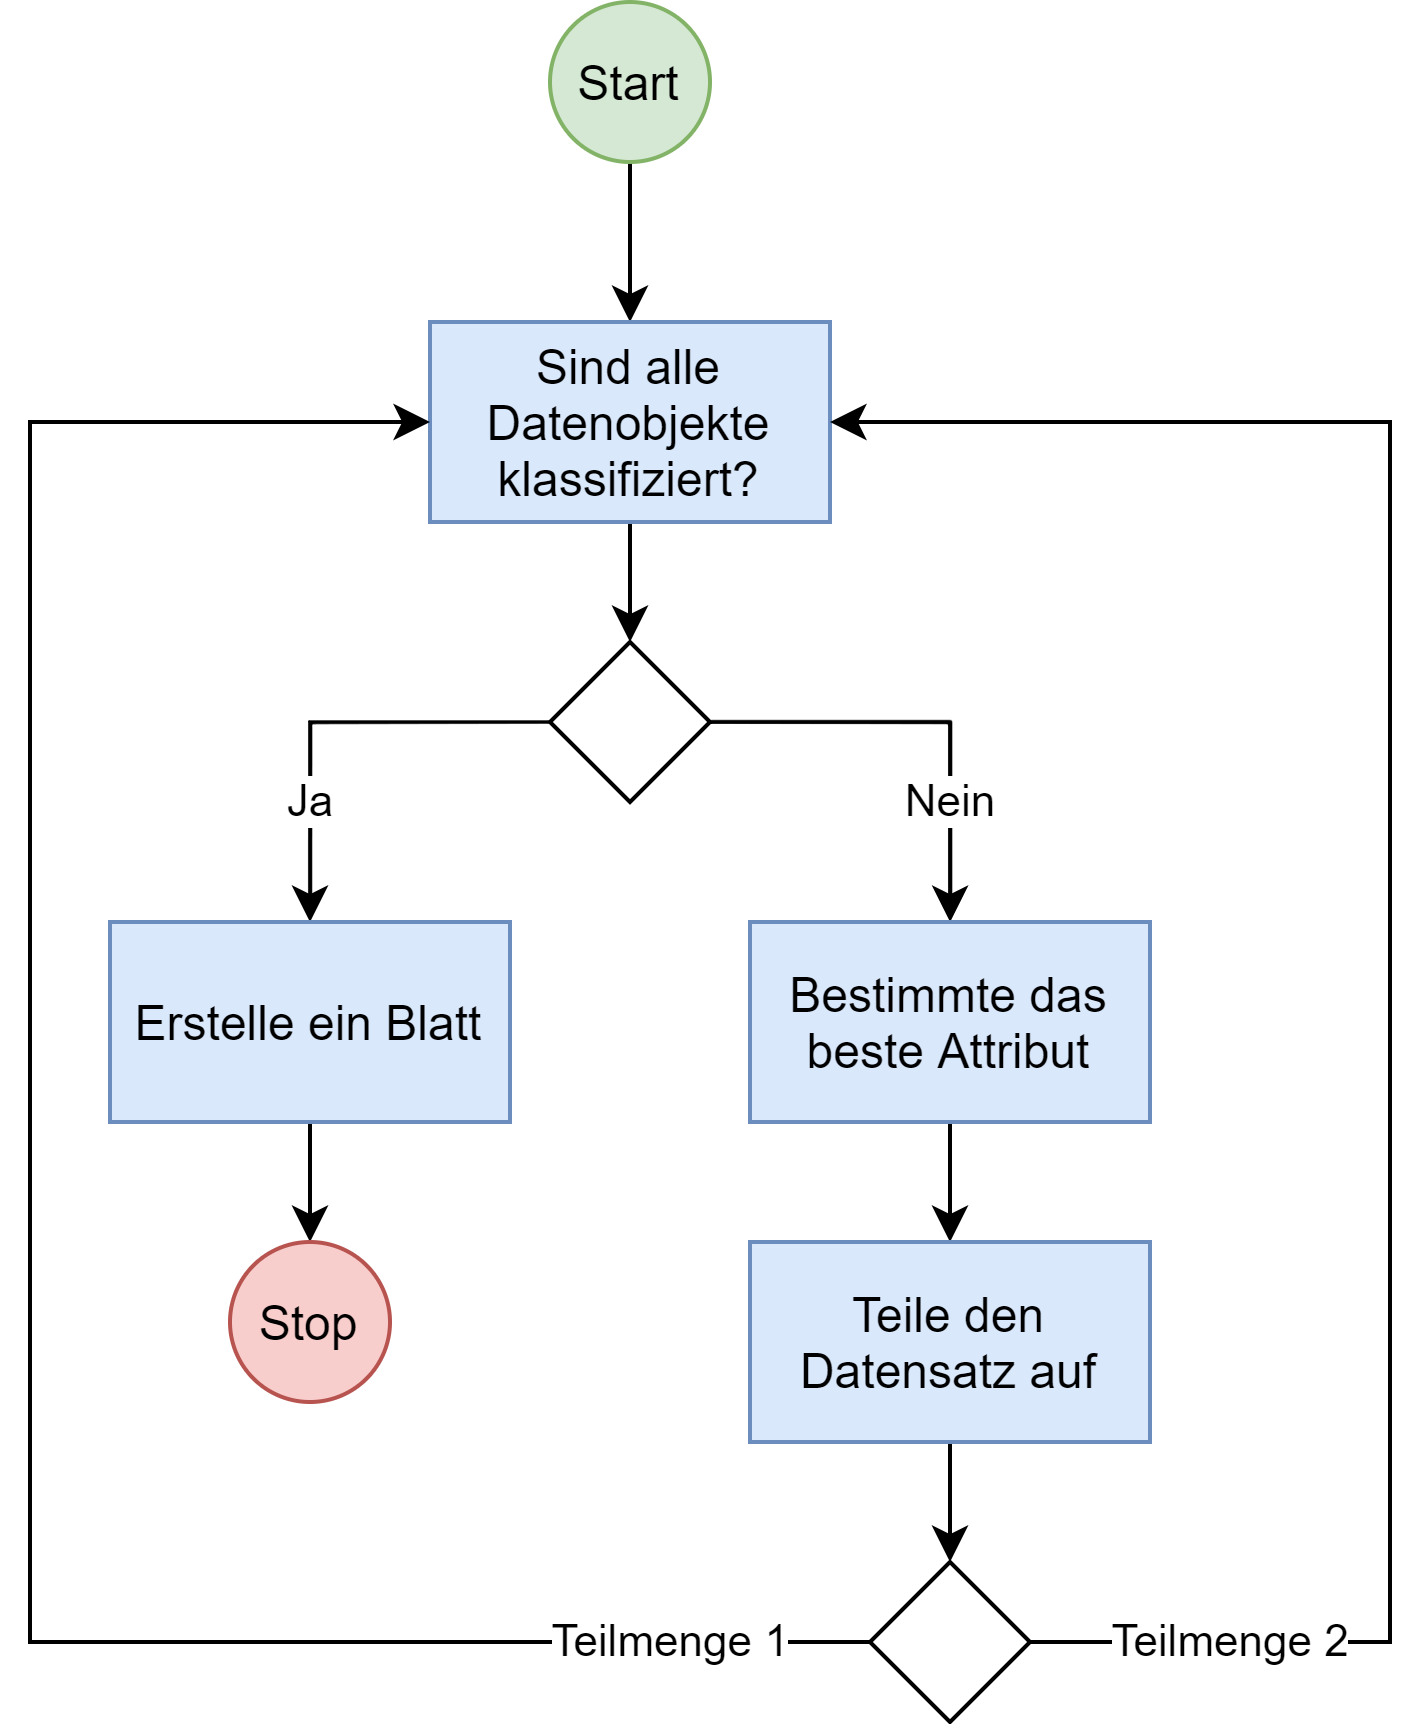
\includegraphics[width=.5\textwidth]{Konzept-Entscheidungsbaum.png}
    \caption{Vereinfachte konzeptionelle Darstellung der Erzeugung eines Entscheidungsbaums \autocite{SebastianManteyPruning:online}}
\end{figure}

Es ist zu beachten dass die Erstellung eines garantiert optimalen Entscheidungsbaums ein NP-vollständiges Problem ist. \autocite{NPComplete} Daher nutzen viele Entscheidungsbaum-Algorithmen einen gierigen Ansatz, was bedeutet dass nur nach der lokal optimalen Entscheidung für jeden Knoten gesucht wird. \autocite{DataMining}\\

Zur Erzeugung eines Entscheidungsbaums wird ein Trainingsdatensatz mit Objekten verwendet, für die bereits eine Klassifikation vorliegt. \autocite{Entschei47:online} Dabei ist zu beachten dass es abhängig vom gewählten Trainingsdatensatz zu sogenanntem \textit{Overfitting} kommen kann. Dies ist zum Beispiel der Fall, wenn ein Datensatz viele Attribute aber nur wenige Datenobjekte besitzt. \autocite{PythonCourseDecisionTrees:online} Entscheidungsbäume die unter \textit{Overfitting} leiden, zeichnen sich dadurch aus, dass sie überangepasst (also gut an den Trainingsdatensatz angepasst) sind und nur schlecht generallisieren. Das bedeutet dass unbekannte reale Daten, die vom Trainingsdatensatz abweichen falsch klassifiziert werden. \autocite{DataMining}
\chapter{Der ID3 Algorithmus}
\label{id3}
Bei ID3 (Iterative Dichotomiser 3) handelt es sich um einen Algorithmus zur Erstellung eines Entscheidungsbaumes welcher von Ross Quinlan entwickelt wurde. \Autocite{QuinlanID3} 

\section{Funktionsweise}
\label{id3:funktionsweise}

\section{Anwendung an einem Beispiel Datensatz}
\label{id3:datensatz}
Zur Veranschaulichung des ID3 Algorithmus wurde ein Datensatz \textit{S} gewählt welcher in Tabelle \ref{table:datensatz-original} dargestellt ist. \Autocite{ImplementationID3}. Dieser Datensatz beinhaltet die Attribute \textit{WEATHER}, \textit{TEMP}, \textit{HUMIDITY} und \textit{WIND} sowie ein Klassifizierung \textit{PLAY}.\\
Hierbei ist die Aufgabe den ID3 Allgorithmus zu nutzen um einen Entscheidungsbaum zu erstellen um vorherzusagen ob das Wetter ermöglicht dass Fußball gespielt werden kann.

\begin{table}[htbp]
    \centering
    \begin{tabular}{cccccc}
        \toprule
        \textbf{DAY} & \textbf{WEATHER} & \textbf{TEMP} & \textbf{HUMIDITY} & \textbf{WIND} & \textbf{PLAY} \\
        \toprule
        1   &Sunny	&Hot	&High	&Weak	&No  \\
        2   &Sunny	&Hot	&High	&Strong	&No  \\
        3   &Cloudy	&Hot	&High	&Weak	&Yes \\
        4   &Rainy	&Medium	&High	&Weak	&Yes \\
        5   &Rainy	&Cold	&Normal	&Weak	&Yes \\
        6   &Rainy	&Cold	&Normal	&Strong	&No  \\
        7   &Cloudy	&Cold	&Normal	&Strong	&Yes \\
        8   &Sunny	&Medium	&High	&Weak	&No  \\
        9   &Sunny	&Cold	&Normal	&Weak	&Yes \\
        10  &Rainy	&Medium	&Normal	&Weak	&Yes \\
        11  &Sunny	&Medium	&Normal	&Strong	&Yes \\
        12  &Cloudy	&Medium	&High	&Strong	&Yes \\
        13  &Cloudy	&Hot	&Normal	&Weak	&Yes \\
        14  &Rainy	&Medium	&High	&Strong	&No  \\
        \bottomrule
    \end{tabular}
    \caption{Beispiel Datensatz \textit{S}}
    \label{table:datensatz-original}
\end{table}

Als erstes werden die Informationsgewinne für die Attribute aus dem Datensatz \textit{S} berechnet. Dabei ergibt sich folgende Übersicht.

\begin{table}[htbp]
    \centering
    \begin{tabular}{lc}
        \textit{IG}(\textit{S}, \textit{WEATHER})  &= 0.246749 \\
        \textit{IG}(\textit{S}, \textit{TEMP})     &= 0.029222 \\
        \textit{IG}(\textit{S}, \textit{HUMIDITY}) &= 0.151835 \\
        \textit{IG}(\textit{S}, \textit{WIND})     &= 0.048127 \\
    \end{tabular}
\end{table}

Da das Attribut \textit{WEATHER} den höchsten Informationsgewinn hat wird es als Knoten bzw. Wurzelknoten gewählt. \textit{WEATHER} besitzt die drei möglichen Ausprägungen \textit{Sunny}, \textit{Cloudy} und \textit{Rainy} für die nun im jeweiligen Iterationschritt eine Teilmenge von \textit{S} erzeugt wird. Daraus ergibt sich zunächst für die Ausprägung \textit{Sunny} folgende Teilmenge $S_{1} = S_{WEATHER=Sunny}$.

\begin{table}[H]
    \centering
    \begin{tabular}{cccccc}
        \toprule
        \textbf{DAY} & \textbf{WEATHER} & \textbf{TEMP} & \textbf{HUMIDITY} & \textbf{WIND} & \textbf{PLAY} \\
        \toprule
        1   &Sunny	&Hot	&High	&Weak	&No  \\
        2   &Sunny	&Hot	&High	&Strong	&No  \\
        8   &Sunny	&Medium	&High	&Weak	&No  \\
        9   &Sunny	&Cold	&Normal	&Weak	&Yes \\
        11  &Sunny	&Medium	&Normal	&Strong	&Yes \\
        \bottomrule
    \end{tabular}
    \caption{Teilmenge $S_{1}$}
    \label{table:datensatz-sunny}
\end{table}

Für $S_{1}$ wird nun rekursiv ein Teilbaum erzeugt wobei die Teilmenge keine der Abbruchbedingungen erfüllt, sodass man nun mit der Berechnung der Informationsgewinne für die Attribute aus $S_{1}$ fortfahren kann. Dabei ergeben sich folgende Werte.

\begin{table}[htbp]
    \centering
    \begin{tabular}{lc}
        \textit{IG}(\textit{S}, \textit{TEMP})     &= 0.570951 \\
        \textit{IG}(\textit{S}, \textit{HUMIDITY}) &= 0.970951 \\
        \textit{IG}(\textit{S}, \textit{WIND})     &= 0.019973 \\
    \end{tabular}
\end{table}

Nun wird das Attribut \textit{HUMIDITY} als Knoten gewählt da es nun den höchsten Informationsgewinn besitzt. Dabei hat \textit{HUMIDITY} die zwei mögliche Ausprägungen \textit{High} und \textit{Normal}. Somit ergeben sich die Teilmengen $S_{1_{HUMIDITY=High}}$ und $S_{1_{HUMIDITY=Normal}}$ aus $S_{1}$.

\begin{table}[H]
    \centering
    \begin{tabular}{cccccc}
        \toprule
        \textbf{DAY} & \textbf{WEATHER} & \textbf{TEMP} & \textbf{HUMIDITY} & \textbf{WIND} & \textbf{PLAY} \\
        \toprule
        1   &Sunny	&Hot	&High	&Weak	&No  \\
        2   &Sunny	&Hot	&High	&Strong	&No  \\
        8   &Sunny	&Medium	&High	&Weak	&No  \\
        \bottomrule
    \end{tabular}
    \caption{Teilmenge $S_{1_{HUMIDITY=High}}$}
    \label{table:datensatz-humidity-high}
\end{table}
\begin{table}[H]
    \centering
    \begin{tabular}{cccccc}
        \toprule
        \textbf{DAY} & \textbf{WEATHER} & \textbf{TEMP} & \textbf{HUMIDITY} & \textbf{WIND} & \textbf{PLAY} \\
        \toprule
        9   &Sunny	&Cold	&Normal	&Weak	&Yes \\
        11  &Sunny	&Medium	&Normal	&Strong	&Yes \\
        \bottomrule
    \end{tabular}
    \caption{Teilmenge $S_{1_{HUMIDITY=Normal}}$}
    \label{table:datensatz-humidity-normal}
\end{table}

Betrachtet man oben genannten Teilmengen fällt sofort auf dass alle Objekte dieser Teilmengen die jeweils die selbe Klassifizierung besitzen. Für $S_{1_{HUMIDITY=High}}$ nämlich die Klassifizierung \textit{No} und für $S_{1_{HUMIDITY=Normal}}$ die Klassifizierung \textit{Yes}. Daher wird für beide Ausprägungen des Knotens \textit{Humidity} ein Blatt erstellt welches jeweils die entsprechende Klassifizierung zugewiesen bekommt. Daraus ergibt sich folgender vorläufiger Teilbaum.

\begin{figure}[htbp]
    \centering
    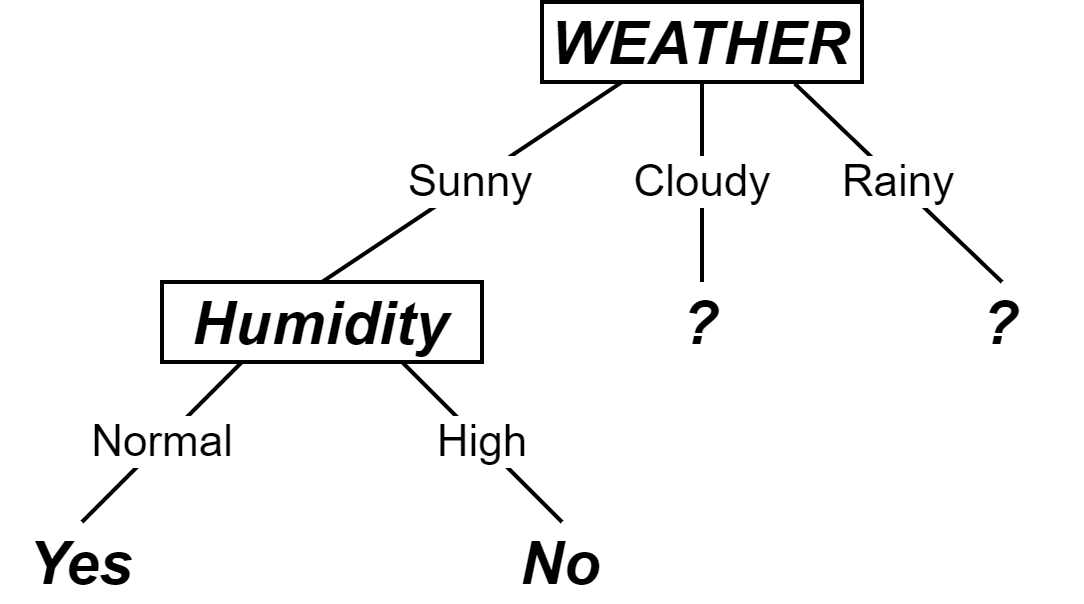
\includegraphics[width=.5\textwidth]{Subtree-Humidity.png}
    \caption{Vorläufiger Teilbaum nachdem \textit{HUMIDITY} klassifiziert wurde}
\end{figure}

Da nun die Ausprägungen des Attributes \textit{HUMIDITY} klassifiziert worden sind fahren wir mit der zweiten Ausprägung von \textit{WEATHER} fort, nämlich \textit{Rainy}. Für diese wird die Teilmenge $S_{2} = S_{WEATHER=Rainy}$ erstellt.

\begin{table}[htbp]
    \centering
    \begin{tabular}{cccccc}
        \toprule
        \textbf{DAY} & \textbf{WEATHER} & \textbf{TEMP} & \textbf{HUMIDITY} & \textbf{WIND} & \textbf{PLAY} \\
        \toprule
        4   &Rainy	&Medium	&High	&Weak	&Yes \\
        5   &Rainy	&Cold	&Normal	&Weak	&Yes \\
        6   &Rainy	&Cold	&Normal	&Strong	&No  \\
        10  &Rainy	&Medium	&Normal	&Weak	&Yes \\
        14  &Rainy	&Medium	&High	&Strong	&No  \\
        \bottomrule
    \end{tabular}
    \caption{Teilmenge $S_{2}$}
    \label{table:datensatz-Rainy}
\end{table}

Für $S_{2}$ wird nun erneut der Informationsgewinn der verbleibenden Attribute berechnet. Zu diesem Zeitpunkt bleiben nur noch die Attribute \textit{TEMP} und \textit{WIND} übrig, da die anderen Attribute bereits verwendet worden sind. Es ergeben sich folgende Werte für den Informationsgewinn.

\begin{table}[htbp]
    \centering
    \begin{tabular}{lc}
        \textit{IG}(\textit{S}, \textit{TEMP})     &= 0.019973 \\
        \textit{IG}(\textit{S}, \textit{WIND})     &= 0.970951 \\
    \end{tabular}
\end{table}

Basierend auf den Informationsgewinnen wird \textit{WIND} als Knoten gewählt. Dieses Attribut besitzt die zwei Ausprägungen \textit{Weak} und \textit{Stong}. Somit ergeben sich die Teilmengen $S_{2_{WIND=Weak}}$ und $S_{2_{WIND=Strong}}$ aus $S_{2}$.

\begin{table}[H]
    \centering
    \begin{tabular}{cccccc}
        \toprule
        \textbf{DAY} & \textbf{WEATHER} & \textbf{TEMP} & \textbf{HUMIDITY} & \textbf{WIND} & \textbf{PLAY} \\
        \toprule
        4   &Rainy	&Medium	&High	&Weak	&Yes \\
        5   &Rainy	&Cold	&Normal	&Weak	&Yes \\
        10  &Rainy	&Medium	&Normal	&Weak	&Yes \\
        \bottomrule
    \end{tabular}
    \caption{Teilmenge $S_{2_{WIND=Weak}}$}
    \label{table:datensatz-wind-weak}
\end{table}

\begin{table}[H]
    \centering
    \begin{tabular}{cccccc}
        \toprule
        \textbf{DAY} & \textbf{WEATHER} & \textbf{TEMP} & \textbf{HUMIDITY} & \textbf{WIND} & \textbf{PLAY} \\
        \toprule
        6   &Rainy	&Cold	&Normal	&Strong	&No  \\
        14  &Rainy	&Medium	&High	&Strong	&No  \\
        \bottomrule
    \end{tabular}
    \caption{Teilmenge $S_{2_{WIND=Strong}}$}
    \label{table:datensatz-wind-strong}
\end{table}

Bei beiden Teilmengen fällt auf dass alle Objekte aus diesen Teilmengen die selbe Klassifizierung aufweisen. An dieser Stelle wird analog zum Vorgehen beim Attribut \textit{HUMIDITY} ein Blatt für die Ausprägungen von \textit{WIND} erstellt. Darus ergibt sich nun folgender Teilbaum.

\begin{figure}[htbp]
    \centering
    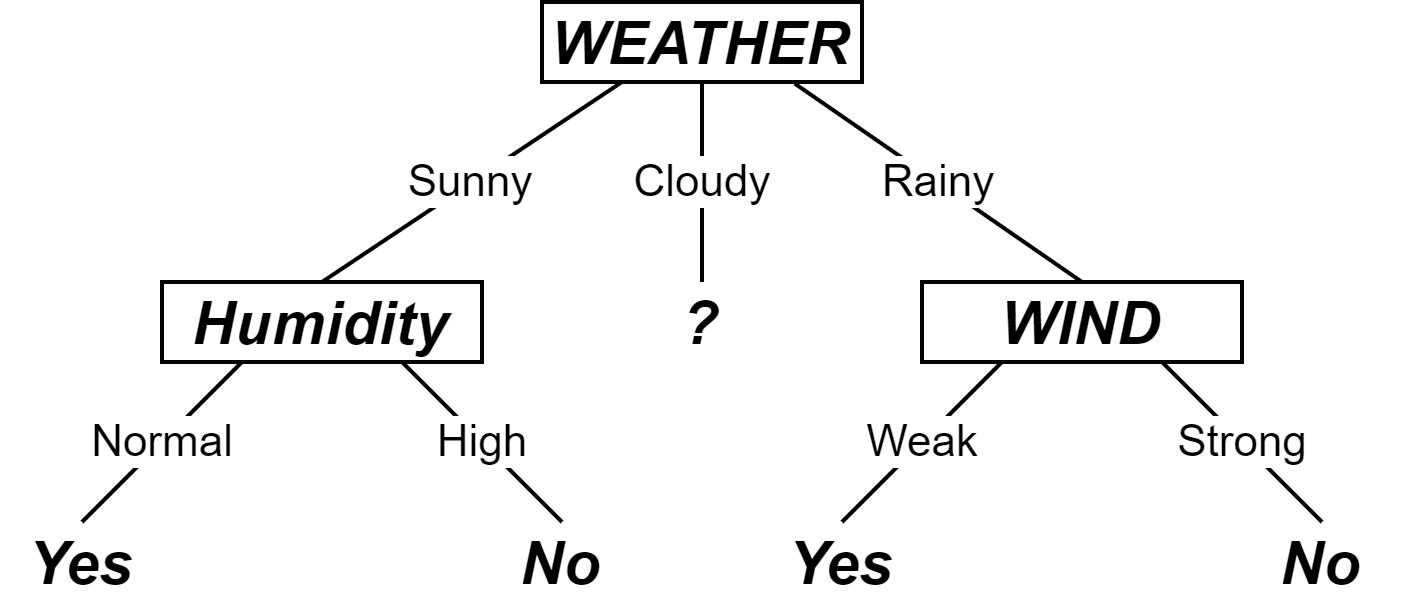
\includegraphics[width=.7\textwidth]{Subtree-Wind.png}
    \caption{Vorläufiger Teilbaum nachdem \textit{WIND} klassifiziert wurde}
\end{figure}

Nachdem also nun die Klassifizierung für das Attribut \textit{WIND} und somit auch für die Ausprägung \textit{Rainy} abgeschlossen ist, bleibt nur noch die Ausprägung \textit{Cloudy} zur Klassifizierung übrig. Basierend darauf ergibt sich folgende Teilmenge $S_{3} = S_{WEATHER=CLoudy}$.

\begin{table}[htbp]
    \centering
    \begin{tabular}{cccccc}
        \toprule
        \textbf{DAY} & \textbf{WEATHER} & \textbf{TEMP} & \textbf{HUMIDITY} & \textbf{WIND} & \textbf{PLAY} \\
        \toprule
        3   &Cloudy	&Hot	&High	&Weak	&Yes \\
        7   &Cloudy	&Cold	&Normal	&Strong	&Yes \\
        12  &Cloudy	&Medium	&High	&Strong	&Yes \\
        13  &Cloudy	&Hot	&Normal	&Weak	&Yes \\
        \bottomrule
    \end{tabular}
    \caption{Teilmenge $S_{3}$}
    \label{table:datensatz-cloudy}
\end{table}

Bei der Betrachtung von $S_{3}$ fällt auf dass alle beinhalteten Objekte die selbe Klassifizierung \textit{Yes} besitzen. Aus diesem Grund wird analog zu der Vorgehensweise bei \textit{WIND} und \textit{HUMIDITY} ein Blatt mit der entsprechenden Klassifizierung erstellt. Somit wird der ID3 Algorithmus beendet und es entsteht der folgende finale Entscheidungsbaum.

\begin{figure}[H]
    \centering
    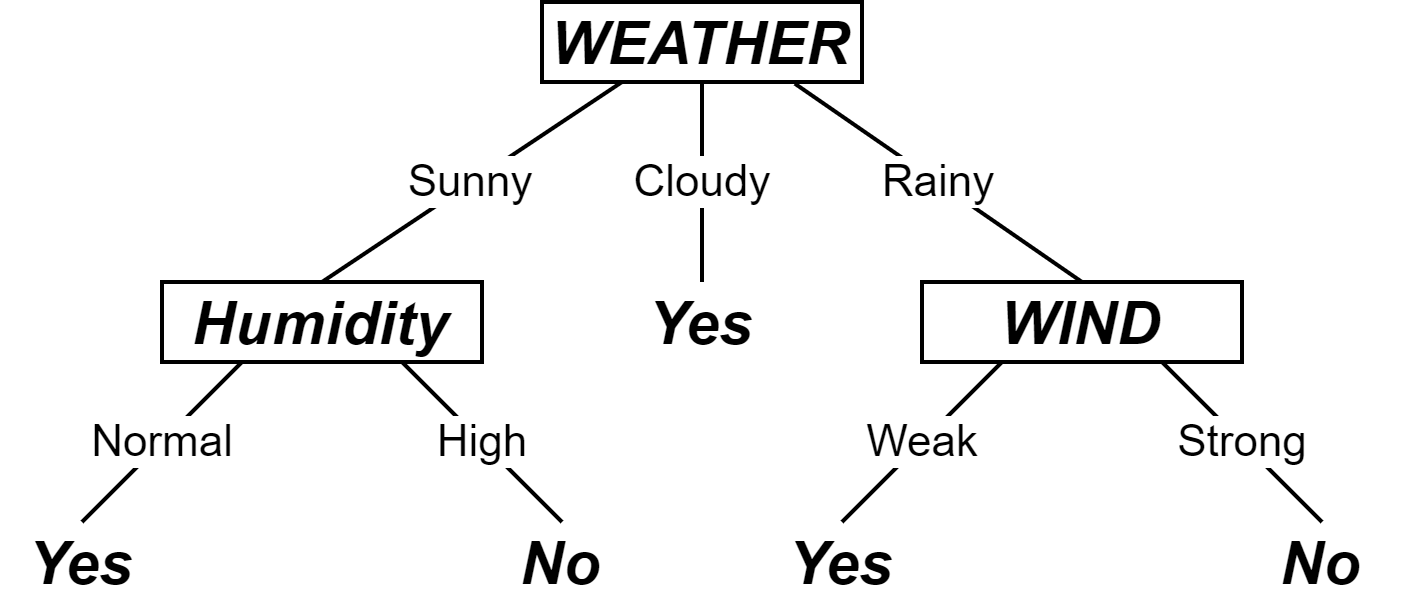
\includegraphics[width=.7\textwidth]{Subtree-Final.png}
    \caption{Finaler Entscheidungsbaum}
\end{figure}

Aus dem oben dargestellten Entscheidungsbaum ergeben sich folgende Regeln für das Spielen. 

\begin{enumerate}
    \item Wenn das Wetter sonnig ist und die Humidität normal, dann kann Fußball gespielt werden. Wenn die Humidität allerdings hoch ist, dann kann kein Fußball gespielt werden. \autocite{ImplementationID3}
    \item Wenn das Wetter bewölkt ist, dann kann Fußball gespielt werden. \autocite{ImplementationID3}
    \item Wenn das Wetter regnerisch ist und der Wind schwach, dann kann Fußball gespielt werden. Falls aber der Wind stark ist, dann kann kein Fußball gespielt werden. \autocite{ImplementationID3}
\end{enumerate}

\pagebreak

\section{Persönliche Implementation}
\label{id3:implementation}
\chapter{Zusammenfassung}
\label{zusammenfassung}

Entscheidungsbäume bieten diverse Vorteile gegenüber anderen Methoden. Einer der offensichtlichsten Vorteile ist die einfache Verständlichkeit und Interpretierbarkeit von Entscheidungsbäumen. \autocite{DataMining} Sie können visualisiert werden und ermöglichen es somit auch Laien mit ihnen zu Arbeiten. \autocite{PythonCourseDecisionTrees:online} Außerdem können Entscheidungsbäume aus Datensätzen erstellt werden die nicht normalisiert sind und sowohl numerische als auch mit kategoriale Attribute enthalten. Dabei können Entscheidungsbäume auch mit sehr großen Datensätzen arbeiten. \autocite{PythonCourseDecisionTrees:online}\\

Aber natürlich besitzen Entscheidungsbäume auch Einschränkungen. So sind sie sind relativ inkonsistent, da bereits kleine Änderungen innerhalb des Trainingsdatensatzes zu weitreichenden Veränderungen des Entscheidungsbaums führen können. \autocite{PythonCourseDecisionTrees:online}\\
Besonders bei Entscheidungsbäumen kann es zu Overfitting kommen wodurch reale Daten falsch klassifiziert werden. Allerdings kann diesem Problem mittels Pruning entgegengewirkt werden. \autocite{DataMining}\\
Wenn Datensätze verwendet werden, die kategorialen Attribute mit einer Vielzahl von möglichen Ausprägungen besitzen, ist der Informationsgewinn in Entscheidungsbäumen zugunsten dieser Attribute ausgelegt.\autocite{PythonCourseDecisionTrees:online}

%%% BIBLIOGRAPHY %%%

\clearpage
\small
\onecolumn
\printbibliography


\end{document}